\documentclass[justified, openany]{tufte-book}

\title{Math Scrapbook}
\author{Uwe Hoffmann}
\publisher{Publisher of This Book}

\usepackage[utf8]{inputenc}
\usepackage[english]{babel}
\usepackage{blindtext}
\usepackage{todonotes}

\hypersetup{colorlinks, pdftitle={Math Scrapbook}}
\setcounter{secnumdepth}{1}
\setcounter{tocdepth}{1}

% turn on numbering for parts and chapters

\usepackage{amsthm, amsmath, amssymb}
\usepackage{setspace, graphicx, enumerate}

\usepackage{stmaryrd}

% For nicely typeset tabular material
\usepackage{booktabs}

\usepackage{listings}
\lstloadlanguages{Haskell}

\usepackage{permute}

\newcommand{\monthyear}{%
  \ifcase\month\or January\or February\or March\or April\or May\or June\or
  July\or August\or September\or October\or November\or
  December\fi\space\number\year
}

\renewcommand{\maketitlepage}{%
  \cleardoublepage%
  {%
  \sffamily%
  \begin{fullwidth}%
  \fontsize{18}{20}\selectfont\par\noindent\textcolor{darkgray}{\allcaps{\thanklessauthor}}%
  \vspace{11.5pc}%
  \fontsize{36}{40}\selectfont\par\noindent\textcolor{darkgray}{\allcaps{\thanklesstitle}}%
  \fontsize{18}{40}\selectfont\par\noindent\textcolor{darkgray}{\allcaps{Notes and Solved Problems}}%
  \vfill%
  \begin{figure*}%
	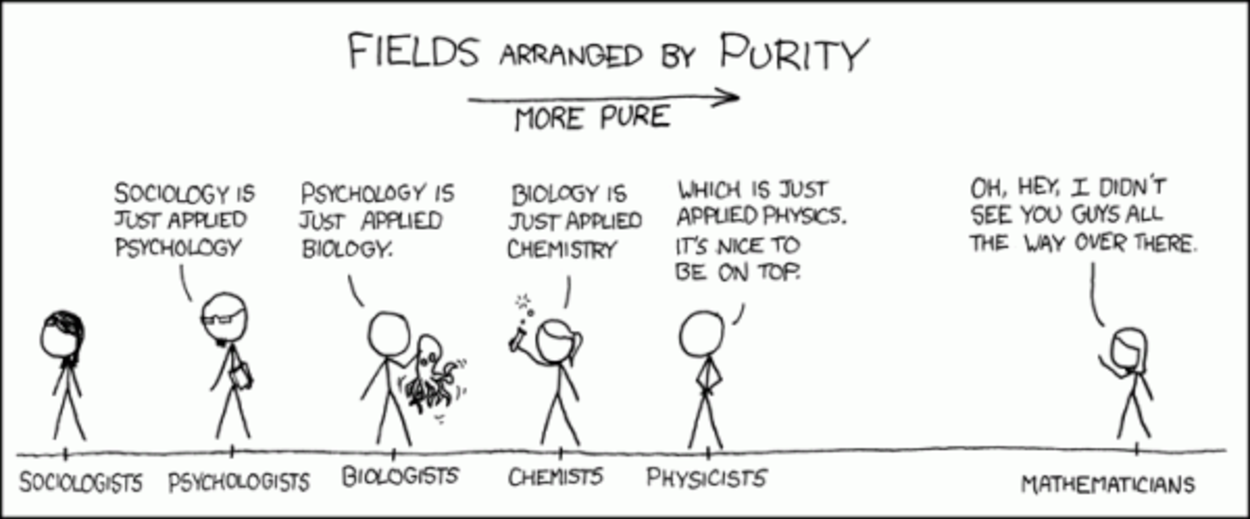
\includegraphics[width=\textwidth]{figs/purity.pdf}%
	\newline\small\url{http://xkcd.com/435/}%
  \end{figure*}%
  \end{fullwidth}%
  }
  \thispagestyle{empty}%
  \clearpage%
}

% For graphics / images
\usepackage{graphicx}
\usepackage{fancyvrb}
\fvset{fontsize=\normalsize}
\usepackage{xspace}

\usepackage{pgf, tikz}
\usetikzlibrary{arrows,automata,decorations.pathmorphing,backgrounds,positioning,fit,petri,shapes.geometric,calc}

\usepackage{units}

\usepackage{bibentry}

\usepackage{tcolorbox}

\usepackage{enumitem}

\usepackage{bm}

\usepackage{mmacells}

\usepackage{pdfpages}

\usepackage{import}

\theoremstyle{plain}% default 
\newtheorem{thm}{Theorem}[chapter] 
\newtheorem{lem}[thm]{Lemma} 
\newtheorem{prop}[thm]{Proposition} 
\newtheorem*{cor}{Corollary} 

\theoremstyle{definition} 
\newtheorem{defn}[thm]{Definition}
\newtheorem{conj}[thm]{Conjecture}
\newtheorem{exmp}[thm]{Example}
\newtheorem{exer}[thm]{Exercise}

\newtheorem{proofpart}{Proof Part}[thm]

\theoremstyle{remark} 
\newtheorem*{rem}{Remark} 
\newtheorem*{note}{Note} 
\newtheorem{case}{Case}
\newtheorem{thminv}{Invariant}[chapter] 

\newtcolorbox{problem}{title={Problem}}

\newenvironment{dedication}
    {\vspace{6ex}\begin{quotation}\begin{center}\begin{em}\begin{large}}
    {\par\end{large}\end{em}\end{center}\end{quotation}}

% Generates the index
\usepackage{makeidx}
\makeindex

\begin{document}
\includepdf[]{figs/cover.pdf}
\frontmatter
\maketitle

\newpage
\begin{fullwidth}
~\vfill
\thispagestyle{empty}
\setlength{\parindent}{0pt}
\setlength{\parskip}{\baselineskip}
Copyright \copyright\ \the\year\ \thanklessauthor

\par Formatted with \LaTeX \xspace using the \url{https://tufte-latex.github.io/tufte-latex/} template.

\par xkcd comics \url{http://xkcd.com}, used under CC license.

\par\smallcaps{uwe@codemanic.com}

\begin{figure}[h]       
    \mbox{
\includegraphics{figs/license/cc.pdf}}   
    \hfill
    \mbox{
\includegraphics{figs/license/by.pdf}}
    \hfill
    \mbox{
\includegraphics{figs/license/nc.pdf}}
    \hfill
    \mbox{
\includegraphics{figs/license/sa.pdf}}
\end{figure}

\par Licensed under the Creative Commons Attribution-NonCommercial-ShareAlike 3.0 Unported License (the ``License''); you may not
use this file except in compliance with the License. You may obtain a copy
of the License at \url{http://creativecommons.org/licenses/by-nc-sa/3.0/deed.en_US}. See the
License for the specific language governing permissions and limitations
under the License.\index{license}

\par\textit{Version \monthyear}
\end{fullwidth}

\newpage
\begin{fullwidth}
\thispagestyle{empty}
\begin{dedication}
Dedicated to my family, in appreciation of their love and support
\end{dedication}
\end{fullwidth}

\chapter{Preface}

Collection of math/cs notes and problems written up over the years for my own amusement. Topics are at the undergraduate college level. Normally notes like these would be written with a pencil in a notebook. LaTeX makes it very easy to produce publishing quality typesetting of mathematical texts, so blame LaTeX for this book. Hopefully others will find some of these notes useful.

I'm an amateur but that hasn't prevented me from enjoying writing these notes just as not being Michael Jordan has never prevented me from enjoying pickup basketball. Describing and explaining has helped me understand the topics involved. Errors and misunderstandings are solely my fault. There is no original content in these notes and I tried to be complete about attributions and citations but if I missed something, I apologize.

Code snippets are mostly in Haskell and Mathematica. I'm not an expert in either but they should work.

\tableofcontents
\cleardoublepage
\mainmatter

\clearpage
\chapter{Airplane Seating}
\subimport{airplane_seating/}{airplane_seating_content.tex}

\clearpage
\chapter{Schr\"oder-Bernstein Theorem}
\subimport{bernstein/}{bernstein_content.tex}

\clearpage
\chapter{Bridge Crossings}
\subimport{bridge/}{bridge_content.tex}

\clearpage
\chapter{Cat vs Dog}
\subimport{catvsdog/}{catvsdog_content.tex}

\clearpage
\chapter{Counting}
\subimport{counting/}{counting_content.tex}

\clearpage
\chapter{Fibolucci}
\subimport{fibolucci/}{fibolucci_content.tex}

\clearpage
\chapter{Grasshopper jumping}
\subimport{grasshopper/}{grasshopper_content.tex}

\clearpage
\chapter{Groovy numbers}
\subimport{groovy/}{groovy_content.tex}

\clearpage
\chapter{Devil's chessboard}
\subimport{hammingcode/}{hammingcode_content.tex}

\clearpage
\chapter{Maximum subsequence}
\subimport{maxsum/}{maxsum_content.tex}

\clearpage
\chapter{No consecutive integers}
\subimport{noconsecutiveints/}{noconsecutiveints_content.tex}

\clearpage
\chapter{Paying a dollar}
\subimport{paying_dollar/}{paying_dollar_content.tex}

\clearpage
\chapter{Penn \& Teller Full Deck of Cards}
\subimport{penn_teller/}{penn_teller_content.tex}

\clearpage
\chapter{Points on circle}
\subimport{pointsoncircle/}{pointsoncircle_content.tex}

\clearpage
\chapter{Prison Cells}
\subimport{prison_cells/}{prison_cells_content.tex}

\clearpage
\chapter{0-1 Sequences}
\subimport{sequences/}{sequences_content.tex}

\clearpage
\chapter{Last three digits before decimal point}
\subimport{threeplussqrtfive/}{threeplussqrtfive_content.tex}

\clearpage
\chapter{How many trailing zeros in $n!$}
\subimport{trailingzeros/}{trailingzeros_content.tex}

\clearpage
\chapter{Twelve Coins}
\subimport{twelvecoins/}{twelvecoins_content.tex}

\clearpage
\chapter{While a}
\subimport{while_a/}{while_a_content.tex}

\begin{fullwidth}
\bibliography{common/math}
\bibliographystyle{plainnat}
\end{fullwidth}

\printindex

\listoftodos

\end{document}

